\documentclass[12pt,a4paper, spanish]{report}
\usepackage[spanish]{babel}
\usepackage[latin1]{inputenc}  % Ambos para solucin de asuntos de idioma
\usepackage[T1]{fontenc}
\usepackage{tocbibind}  % Bibliografa en el indice
\usepackage{titlesec}  % Posibilidad de editar los formatos de chapter y section
%\usepackage{times}  % Fuente de letras
\usepackage{amsmath,amssymb,mathrsfs,mathptmx}  % Matemticas varias
\usepackage{hyperref} % Para escribir URLs



% --- Arreglos varios para la inclusion de imgenes
%\usepackage[pdftex]{graphicx}
%\usepackage[dvips]{graphicx}
\usepackage{graphicx}
\usepackage{epstopdf}
\usepackage{float}
\usepackage{subfigure}
%\usepackage{subfig}
\usepackage{wrapfig}
\usepackage[usenames,dvipsnames]{color}
\DeclareGraphicsExtensions{.png,.jpg,.pdf,.mps,.gif,.bmp, .eps}


	

\usepackage{multirow}
\usepackage{multicol}
\usepackage{tabulary}
\usepackage[table]{xcolor}
\usepackage{color}
\usepackage{listings}
%\usepackage{subfloat}
\usepackage{tikz}

\setcounter{secnumdepth}{3}
\setcounter{tocdepth}{3}


% --- Para las dimensiones de los mrgenes etc
\frenchspacing \addtolength{\hoffset}{-1.5cm}
\addtolength{\textwidth}{3cm} \addtolength{\voffset}{-2.5cm}
\addtolength{\textheight}{4cm}
% --- Para el encabezado
\usepackage{fancyhdr}
\fancyhead[R]{2012}\fancyhead[L]{enCuadro} \fancyfoot[C]{\thepage}
\pagestyle{fancy}

% --- Formato de la etiqueta Chapter
%\newcommand{\bigrule}{\titlerule[0.5mm]}
%\titleformat{\chapter}[display]{\bfseries\Huge}
%{\Large\chaptertitlename\ \Large\thechapter}
%{0mm} {\filleft} [\vspace{0.5mm} \bigrule]

\titleformat{\chapter}[display]
{\normalfont\Large\filcenter}
{\titlerule[1pt]%
\vspace{1pt}%
\titlerule
\vspace{1pc}%
\LARGE\MakeUppercase{\chaptertitlename} \thechapter}
{1pc}
{\titlerule
\vspace{1pc}%
\Huge}

%-------------------------

\begin{document}
% Esto es para que se muestren todas las referencias aunque no se citen:
\nocite{*}

\renewcommand{\tablename}{Tabla}
\renewcommand{\theenumi}{\Roman{enumi}}
\renewcommand{\labelenumi}{[\textbf{\theenumi}]}
\renewcommand{\thefootnote}{\arabic{footnote}}
% --- Modificacin de entornos enumerate
\renewcommand{\theenumi}{\roman{enumi}}
\renewcommand{\labelenumi}{\theenumi)}
% --- Modificacin de entornos enumerate

% --- Para hacer highlights
\newcommand{\highlAmarillo}[1]{\colorbox{yellow}{#1}}
\newcommand{\highlVerde}[1]{\colorbox{green}{#1}}
\newcommand{\highlRojo}[1]{\colorbox{red}{#1}}

%



\chapter{Casos de Uso}
\label{chap: casoUso}
\section{Introducci�n}
En este cap�tulo se presentan los distintos casos de uso que se implementaron con el fin de integrar los algoritmos comentados en cap�tulos anteriores en peque\~nas aplicaciones que funcionen \textit{de punta a punta}. Se busc� resolver individualmente los diferentes desaf�os t�cnicos que una aplicaci�n real de realidad aumentada para museos puede llegar a tener. Estas �ltimas no ser�n m�s que una combinaci�n guionada de cada uno de estos casos de uso.\\

A lo cargo del cap�tulo se ver�n entonces los tres casos de uso implementados: ``interactividad'', ``video'' y ``modelos''. El primero presenta un modelo simple sobre el marcador que responde a toques con cierto movimiento y un audio en particular, el segundo soluciona el problema de proyectar un video sobre el marcador de forma consistente con el movimiento del usuario. El �ltimo caso de uso muestra c�mo es posible importar modelos a ISGL3D de manera de lograr realidades aumentadas mucho m�s interesantes que si tan s�lo se hicieran con las primitivas del \textit{framework}, por detalles ver Cap�tulo \ref{chap: render}.

% -------------------------------- |Caso de uso INTERACTIVIDAD| ------------------------------------

\section{Caso de uso ``interactividad''}
\label{sec: casoUso1}
\subsection{Comentarios sobre el caso de uso}
En este caso de uso se implementa la parte interactiva de la aplicaci�n. Al enfocar el marcador, se puede ver un cubo sobre el $QlSet$ de la esquina superior izquierda. Ver Figura \ref{fig:CasoUso1}. Si el cubo es tocado a trav�s de la pantalla del dispositivo, este se anima y se reproduce un audio que indica la posici�n del cubo en el instante de ser presionado. Inmediatamente despu�s, es desplazado hacia el $QlSet$ de la esquina superior derecha. Nuevamente, si el cubo es tocado a trav�s de la pantalla del dispositivo, este se anima y se reproduce un audio que indica la posici�n del cubo en el instante de ser presionado. Inmediatamente despu�s, este se desplaza hacia el $QlSet$ restante. Lo anterior suceder� de forma c�clica, cada vez que se presione sobre el modelo.\\ 

Esta funcionalidad es fundamental si lo que se quiere implementar es por ejemplo una audiogu�a interactiva. Podr�a pensarse una aplicaci�n en la que el cubo anterior se reemplace por flechas 3D, y que estas sean ubicadas conjuntamente en distintas partes de una obra. Entones, al seleccionar cada una de las flechas, se podr�a reproducir un audio con informaci�n referente a esa zona o punto en particular.\\ 


\begin{figure}[h!]
\centering
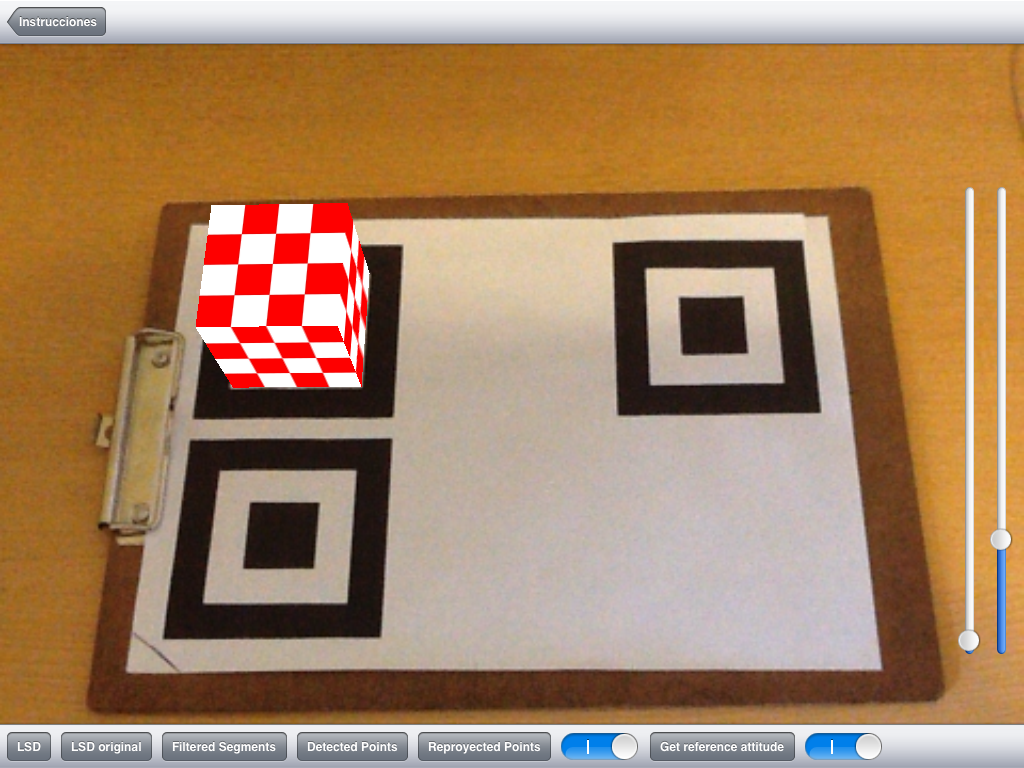
\includegraphics[scale=0.3]{figs_casosuso/CasoUso1.PNG}
\caption{Captura de pantalla del caso de uso ``interactividad'. Se puede ver al cubo apoyado sobre el $QlSet$ de la esquina superior izquierda y los diferentes controles que ayudan a la depuraci�n del c�digo.}
\label{fig:CasoUso1}
\end{figure}

Esta aplicaci�n tambi�n se utiliz� con fines de \textit{debugging} o depuraci�n de la integraci�n de cada uno de los bloques. Se le agregaron las siguientes funcionalidades:
\begin{itemize}
\item La posibilidad de ver dibujados sobre la imagen los segmentos detectados por LSD. En sus versiones original y opimizada.
\item La posibilidad de ver dibujados sobre la imagen los segmentos filtrados pertenecientes al marcador. As� como tambi�n las esquinas detectadas de cada uno de los cuadril�teros que lo forman.
\item La posibilidad de variar el umbral utilizado para el filtrado de segmentos. 
\item La posibilidad de ver las esquinas de cada uno de los cuadril�teros que forman al marcador reproyectadas seg�n la pose del dispositivo obtenida.
\item La posibilidad de prender o apagar el filto de Kalman.
\item La posibilidad de aumentar o disminuir el ruido de medici�n del filtro de Kalman.
\item La posibilidad de elegir si usar o no la fusi�n de la estimaci�n de pose con los sensores. 
\end{itemize} 

%\begin{figure}[h!]
%\centering
%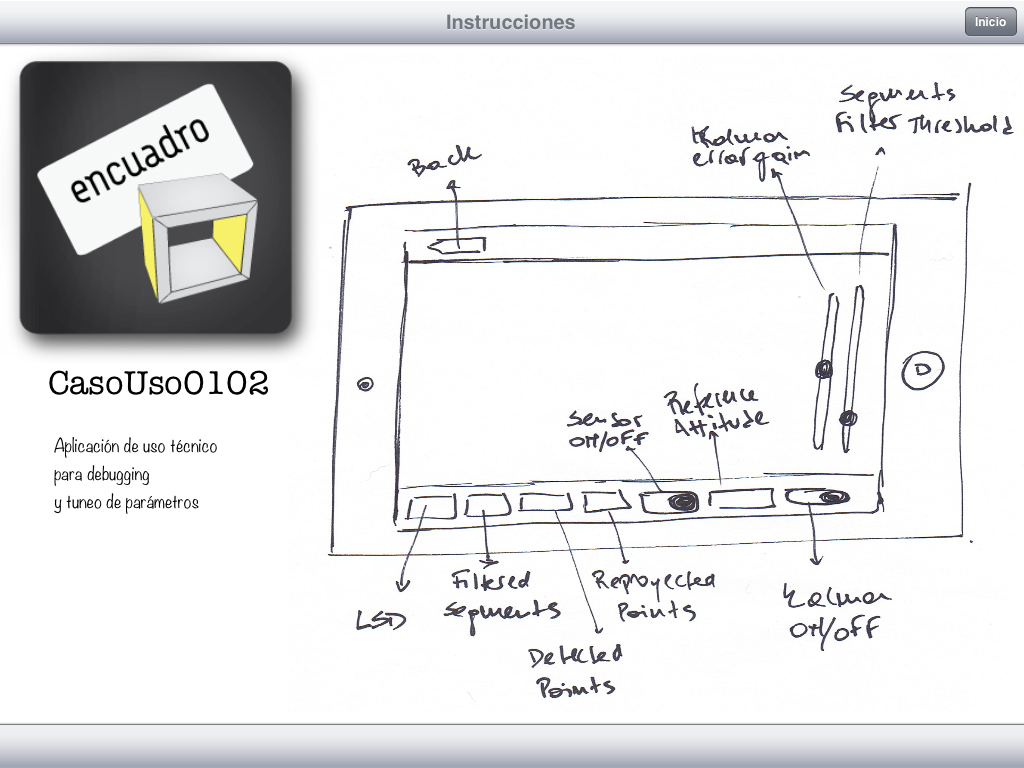
\includegraphics[scale=0.35]{figs_casosuso/CasoUso1ini}
%\caption{Pantalla inicial de caso de uso 1, en esta pantalla se explica como funciona la interfaz de usuario }
%\label{fig:CasoUso1ini}
%\end{figure}



En la Figura \ref{fig:CasoUso1} tambi�n se puede ver c�mo es la interfaz de usuario de este caso de uso, en donde se puede elegir entre todas las funcionalidades anteriores. El mismo fue fundamental para evaluar el desempe\~no de los algoritmos utilizados funcionando en tiempo real. Gracias a estas funcionalidades se pudieron definir las condiciones para las cuales el conjunto de todos los bloques funciona mejor. Se fue variando la distancia al marcador y se ajust� el umbral para el filtro de segmentos. Adem�s, se pudieron ajustar los par�metros del filtro de Kalman y se pudo comparar el desempe\~no de la estimaci�n de pose utilizando solamente informaci�n de la c�mara con el resultado obtenido de la fusi�n de sensores. Fue en este caso de uso que se evalu� cualitativamente el desempe\~no de la versi�n optimizada de LSD, respecto del de la versi�n original. \\

Si bien todas estas pruebas y ajustes si hicieron previamente en una computadora y con im�genes de prueba, fue necesario contar con una aplicaci�n en la que se pudiera ver sobre el dispositivo al conjunto de los algoritmos funcionando en tiempo real.  
\subsection{Detalles constructivos}
\subsubsection{Objetos ISGL3D interactivos}

La manera de agregar interactividad a un nodo ISGL3D es bastante sencilla. En primer lugar, debe configurarse su propiedad \textit{interactive} de forma positiva y luego se le debe ejecutar el m�todo \textit{addEvent3DListener}:
\footnotesize
\begin{verbatim}
Isgl3dTextureMaterial * material = [Isgl3dTextureMaterial 
materialWithTextureFile:@"red_checker.png" shininess:0.9 
precision:Isgl3dTexturePrecisionMedium repeatX:NO repeatY:NO];
 
Isgl3dCube* cubeMesh = [Isgl3dCube  meshWithGeometry:60 height:60 depth:60 nx:40 ny:40];
        
Isgl3dNode * _cubito = [self.scene createNodeWithMesh:cubeMesh andMaterial:material];

_cubito.interactive =YES;

[_cubito1 addEvent3DListener:self method:@selector(objectTouched:) forEventType:TOUCH_EVENT];
\end{verbatim}
\normalsize
En el c�digo anterior, primero se crea un nodo llamado ``$\_$cubito'' con la primitiva de un cubo y cierto material. Luego, se indica que s� se quiere que dicho nodo tenga interactividad y finalmente se lo configura para que cuando ``$\_$cubito'' reciba eventos del tipo \textit{TOUCH$\_$EVENT}, o lo que es lo mismo, cuando se lo toque; se ejecute el m�todo \textit{objectTouched}, definido en la misma clase que esta escrito el c�digo (\textit{self}).\\

En este caso de uso lo que se hizo en \textit{objectTouched} no fue m�s que cambiar la posici�n del cubo en la escena y reproducir un audio dependiente de la posici�n del mismo.\\

\subsubsection{Reproducci�n de audio en Objective-C}

Para reproducir audios en Objective-C primero la clase en la que se quiere reproducir el audio debe importar el \textit{framework AVFoundation} y luego debe implementar el protocolo \textit{AVAudioPlayerProtocol}. El c�digo que se debe escribir es el sigiuente:
\footnotesize
\begin{verbatim}
NSURL *url =[NSURL fileURLWithPath:[NSString stringWithFormat:@"%@/%@", 
         [[NSBundle mainBundle] resourcePath],audio.mp3]];

AVAudioPlayer * audioPlayer =[[AVAudioPlayer alloc] initWithContentsOfURL:url error:nil];

audioPlayer.numberOfLoops=0;
   
audioPlayer.delegate = self;

[audioPlayer play];

\end{verbatim}
\normalsize
En la primera l�nea se genera un \textit{url} que indica cu�l es el audio a reproducir y luego se le asigna a una instancia de la clase \textit{AVAudioPlayer}. Se dice que no se quiere reproducir el audio en bucle, se asigna a la clase en la que se esta escribiendo el c�digo como la delegada de \textit{audioPlayer}, una instancia de \textit{AVAudioPlayer,} y finalmente se le da inicio al audio. Luego de reproducido el audio, se ejecuta autam�ticamente el m�todo de firma:
\footnotesize
\begin{verbatim}
- (void)audioPlayerDidFinishPlaying:(AVAudioPlayer *)player successfully:(BOOL)flag;
\end{verbatim}
\normalsize
En este c�digo es en donde se indica que la pr�xima vez que se presione sobre el cubo, se querr� reproducir un audio distinto.\\

\subsubsection{Dibujar en ISGL3D}

Lo que se hizo fue crear una clase nueva, del tipo \textit{UIVIew}, a la que se la llam� ``claseDibujar''. Esta fue agregada como \textit{subView} de la \textit{view} en donde se muestra el video por detr�s de lo que dibuja ISGL3D. Dicha clase se configur� para que fuera transparente y del mismo tama\~no que la pantalla del \textit{iPad}. \textit{claseDibujar} cuenta con una cantidad de propiedades a las que se les asignan los diferentes puntos o segmentos que se quieren dibujar; son del tipo ``puntero a entero'' y ``puntero a \textit{float}'' respectivamente. Luego, un m�todo llamado \textit{drawRect} es el que se encarga de dibujar cada uno de los puntos y segmentos. Los puntos se dibujan con las siguientes l�neas de c�digo:
\footnotesize
\begin{verbatim}
CGContextRef context = UIGraphicsGetCurrentContext();

CGContextStrokeRect(context, CGRectMake(punto_X, punto_Y, 4, 4));
\end{verbatim}
\normalsize
En la primera l�nea de c�digo se crea un contexto. Un contexto contiene ciertos par�metros y toda la informaci�n especifica del dispositivo, requerida para poder dibujar. En la segunda l�nea se dibuja cada punto como un rect�ngulo centrado en el punto en cuesti�n y con 4 p�xeles de ancho y largo. Los segmentos se dibujan con las siguientes l�neas de c�digo:
\footnotesize
\begin{verbatim}
CGContextRef context = UIGraphicsGetCurrentContext();

CGContextStrokeLineSegments(context, puntos, 2);
\end{verbatim}
\normalsize
En la primera l�nea de c�digo se crea un contexto (este paso puede saltearse si ya fue creado anteriormente), y en la segunda se dibuja la l�nea. La variable ``puntos'' es un arreglo de dos variables del tipo \textit{CGPoint}, cada una de ellas tiene dos valores en precisi�n simple correspondientes a las coordenadas de un punto. Adem�s, se le configura al segmento una anchura de 2 p�xeles. \\

Finalmente, es bueno aclarar que \textit{claseDibujar} se instancia y se destruye cuadro a cuadro; el m�todo \textit{drawRect} se invoca cada vez que se instancia la clase.\\

% -------------------------------- |Caso de uso VIDEO | ------------------------------------

\section{Caso de uso ``video''}
\subsection{Comentarios sobre el caso de uso}
Este caso de uso proyecta un video sobre el $QlSet$ de la esquina superior izquierda del marcador de manera consistente con la pose del dispositivo. Ver Figura \ref{fig:CasoUso2}. La aplicaci�n de esta soluci�n t�cnica es directa. Tan s�lo ajustando un par de par�metros el video podr�a ser proyectado dentro del marco de un cuadro, sobre uno de sus extremos, sobre una pared blanca o incluso sobre un mapa. Esto puede ser de gran inter�s para un museo, por ejemplo como complemento a una audiogu�a. A continuaci�n se explican brevemente algunos detalles t�cnicos que fue necesario solucionar para lograr implementar este caso de uso.\\
	
\begin{figure}
\centering
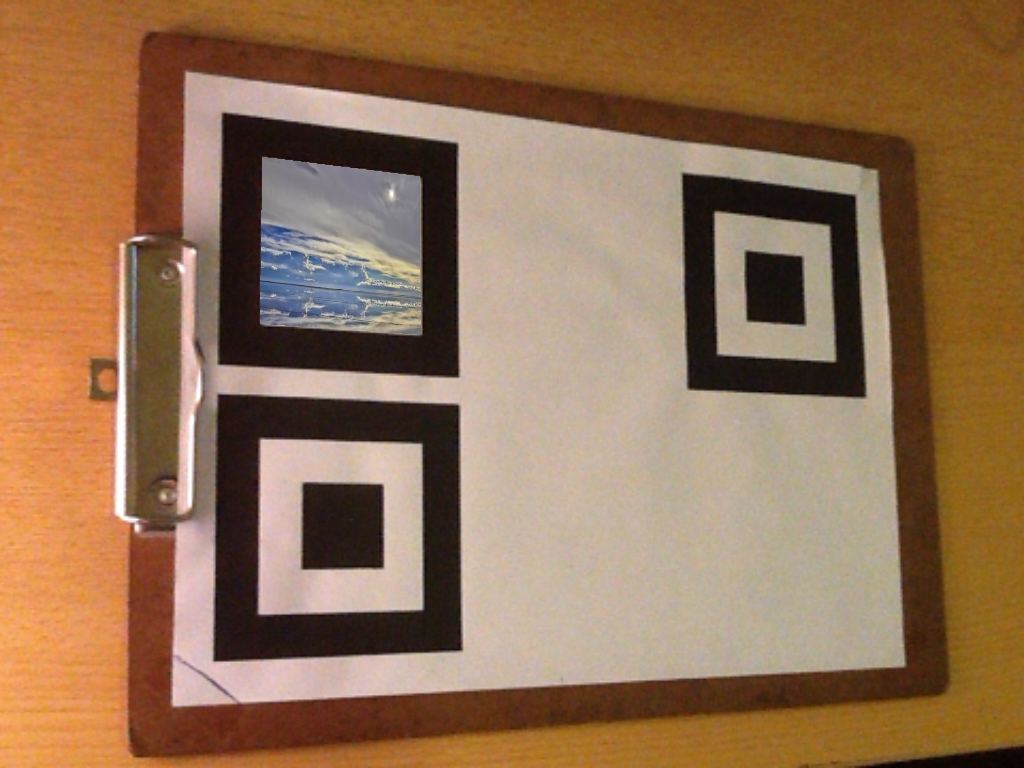
\includegraphics[scale=0.3]{figs_casosuso/CasoUso2}
\caption{Captura de pantalla del caso de uso ``video''. Se puede ver al video proyectado sobre el $QlSet$ de la esquina superior izquierda}
\label{fig:CasoUso2}
\end{figure}

\subsection{Detalles constructivos}
El desaf�o t�cnico es, dados 4 puntos din�micos cualesquiera sobre la pantalla, poder repdocucir un video cuyas esquinas se ajusten a esos 4 puntos. Por lo tanto, en la implementaci�n del presente caso de uso, de toda la l�gica de estimaci�n de pose, solamente se hace uso de los bloques de detecci�n, filtrado y determinaci�n de correspondencias. En particular, no se utiliza el algoritmo POSIT visto en el Cap�tulo \ref{ch: posit}.  Teniendo entonces detectados los l�mites dentro de los que se quiere reproducir el video, parecer�a que el problema est� resuelto, pues s�lo basta con ubicar al video dentro de los mismos. Sin embargo, \textit{Xcode} no permite posicionar en forma directa una \textit{view} (que ser� la que embeba al video) tomando como l�mites cuatro puntos cualesquiera.\\

Si s�lo se quiere reproducir un video, y no se quiere procesar su contenido, la soluci�n m�s simple es utilizar la clase \textit{MPMoviePlayerController} que hereda de \textit{NSObject}. Una alternativa similar es hacer uso de la clase \textit{MPMoviePlayerViewController} que hereda de \textit{UIViewController} y tiene como �nica propiedad una del tipo \textit{MPMoviePlayerController}. \textit{MPMoviePlayerController} tiene como atributo una \textit{view}, del tipo \textit{UIView}, y son las esquinas de este atributo a las que se las quiere posicionar sobre 4 de los 36 puntos detectados por el filtro. La clase \textit{UIView} tiene un atributo \textit{frame} que es del tipo \textit{CGRect}:
\begin{verbatim}
theMovie.view.frame = CGRectMake(0, 0, 60, 60);
\end{verbatim}
En el c�digo anterior \textit{theMovie} es del tipo \textit{MPMoviePlayerController}. De esta manera, parecer�a que los videos solamente pueden ser reproducidos sobre rect�ngulos y no sobre cualquier cuadril�tero gen�rico. Sin embargo, algo que s� se les puede hacer a las instancias de la clase \textit{UIView} es una transformaci�n af�n o incluso, de forma m�s gen�rica, una homograf�a. \\

\subsection{\textit{CGAffineTransform} y \textit{CATransform3D}}
La clase \textit{UIView} tiene una propiedad llamada \textit{transform} que es del tipo \textit{CGAffineTransform}. Las primeras letras de esta clase  (\textit{CG}) refieren a la API \textit{\textbf{Core Graphics} }utilizada ampliamente como herramienta para resolver problemas de \textit{rendering} y cualquier tipo de transformaci�n en 2D.\\

La clase \textit{UIView} adem�s tiene una propiedad llamada \textit{layer} que es del tipo \textit{CALayer} y que permite realizar transformaciones del tipo	 \textit{CATransform3D}. Las primeras letras de estas dos clases  (\textit{CA}) refieren a la API \textit{\textbf{Core Animation}} que es utilizada para generar animaciones y transformaciones sobre objetos 3D solamente indicando un punto inicial y final para el objeto (tambi�n es posible agregar efectos para la transici�n). En definitiva, para resolver el problema del caso de uso existen \textit{a priori} dos alternativas posibles: \textit{CGAffineTransform} y \textit{CATransform3D}.\\

Se pueden generar f�cilmente instancias de transformaciones afines invocando la siguiente funci�n:
\begin{verbatim}
CGAffineTransform CGAffineTransformMake (
   CGFloat a,
   CGFloat b,
   CGFloat c,
   CGFloat d,
   CGFloat tx,
   CGFloat ty
);
\end{verbatim}
que toma 6 \textit{CGFloats} (n�meros reales en coma flotante y precisi�n simple), y crea una \textit{CGAffineTransform}, donde cada uno de los valores anteriores se corresponde con los elementos de una matriz transformaci�n af�n de la siguiente manera\footnote{V�ase que en este caso \textit{Apple} expresa la matriz af�n de forma traspuesta a lo que se comunmente acostumbra.}:
\[
\left( \begin{array}{ccc}
a & b & 0 \\ 
c & d & 0 \\
t_{x} & t_{y} & 1 
\end{array} \right)
\]
As� entonces, de los 9 valores de la matriz, 2 de ellos son nulos por tratarse de una transformaci�n af�n y otro de ellos es un factor de escala de valor constante 1. Resolviendo el sistema como se muestra en la Secci�n \ref{sec: resHomo} y obteniendo los restantes 6 valores, se le puede asignar transformaciones a la propiedad \textit{transform} y realizar la trasnformaci�n deseada. Sin embargo, una transformaci�n af�n preserva colinealidad y realaciones entre distancias; y lo que realmente se necesita en este caso es una transformaci�n proyectiva. Se decidi� entonces estudiar la posibilidad de utilizar una \textit{CATransform3D}.\\

Una \textit{CATransform3D} se define de la siguiente manera:
\begin{verbatim}
struct CATransform3D
{
CGFloat m11, m12, m13, m14;
CGFloat m21, m22, m23, m24;
CGFloat m31, m32, m33, m34;
CGFloat m41, m42, m43, m44;
};
typedef struct CATransform3D;
\end{verbatim}
donde $m_{ij}$ corresponde al elemento de la matriz ubicado en la fila $i$ y la columna $j$. As� entonces, conociendo los valores que debe tomar la homograf�a, tambi�n es posible completar los elementos de esta matriz $4\times 4$ y asignarle la transformaci�n a la propiedad \textit{layer} de cualquier objeto del tipo \textit{UIView}. Dem�s esta decir que una transformaci�n 3D es algo bastante m�s gen�rico que una transformaci�n proyectiva; pero si se anulan algunas entradas de la matriz, es posible lograr el tipo de transformaci�n que se busca. En particular, la coordenada \textit{z} debe ser nula:
\[
\left( \begin{array}{cccc}
m_{11} & m_{12} &    0   & m_{14}\\ 
m_{21} & m_{22} &    0   & m_{24}\\
   0   &    0   &    1   &    0  \\
m_{41} & m_{42} &    0   & m_{44}
\end{array} \right)
\]
donde tambi�n en este caso se asume el valor unitario para $m_{44}$ por ser tan s�lo un factor de escala. Al igual que para la transformaci�n af�n, resolviendo la homograf�a como se ve en la Secci�n \ref{sec: resHomo} se obtienen los 8 valores restantes de la matriz.

\subsection{Resoluci�n de Homograf�a}
\label{sec: resHomo}
A continuaci�n se plantea la resoluci�n del sistema de ecuaciones que, dados 4 punto correspondientes entre 2 planos, halla los par�metros de la homograf�a que los relaciona. La explicaci�n que sigue es un caso particular de la del m�todo DLT explicado en la Secci�n \ref{subsec: DLT}. Esta transformaci�n proyectiva se puede expresar en forma matricial, en coordenadas homog�neas, de la siguiente manera:
\[
\left( \begin{array}{ccc}
\textbf{H}_{11} & \textbf{H}_{12} & \textbf{H}_{13} \\ 
\textbf{H}_{21} & \textbf{H}_{22} & \textbf{H}_{23} \\
\textbf{H}_{31} & \textbf{H}_{32} & \textbf{H}_{33} 
\end{array} \right)
\left( \begin{array}{c}
x \\ 
y \\
s
\end{array} \right)
=
\left( \begin{array}{c}
U \\
V \\
P
\end{array} \right)
\]
donde la matriz $\textbf{H}_{3x3}$  representa la transformaci�n homogr�fica, el vector $(x,y,s)^t$  representa los puntos de referencia y el vector $(U,V,P)^t$  respresenta los puntos transformados. Asumiendo un valor unitario para las coordenadas $s$ y $P$ la resoluci�n del sistema se simplifica mucho y no se pierde generalidad. Imponiendo esto entonces, el sistema anterior se puede expresar de la siguiente forma:
\begin{equation}\label{eq_1}
x\textbf{H}_{11} + y\textbf{H}_{12} + \textbf{H}_{13} = U
\end{equation}
\begin{equation}\label{eq_2}
x\textbf{H}_{21} + y\textbf{H}_{22} + \textbf{H}_{23} = V
\end{equation}
\begin{equation}\label{eq_3}
x\textbf{H}_{31} + y\textbf{H}_{32} + \textbf{H}_{33} = 1
\end{equation}
Multiplicando la ecuaci�n \eqref{eq_3} por $U$ e igual�ndola a la ecuaci�n \eqref{eq_1} se obtiene lo siguiente:
\begin{equation}
x\textbf{H}_{11} + y\textbf{H}_{12} + \textbf{H}_{13} = xU\textbf{H}_{31} + yU\textbf{H}_{32} + U\textbf{H}_{33}
\end{equation}
o lo que es lo mismo:
\begin{equation}\label{eq_4}
x\textbf{H}_{11} + y\textbf{H}_{12} + \textbf{H}_{13} - xU\textbf{H}_{31} - yU\textbf{H}_{32} - U\textbf{H}_{33}=0
\end{equation}
Procediendo de manera an�loga y multiplicando la ecuaci�n \eqref{eq_3} por $V$ e igual�ndola a la ecuaci�n \eqref{eq_2} se obtiene lo siguiente:
\begin{equation}
x\textbf{H}_{21} + y\textbf{H}_{22} + \textbf{H}_{23} = xV\textbf{H}_{31} + yV\textbf{H}_{32} + V\textbf{H}_{33}
\end{equation}
o lo que es lo mismo:
\begin{equation}\label{eq_4}
x\textbf{H}_{21} + y\textbf{H}_{22} + \textbf{H}_{23} - xV\textbf{H}_{31} - yV\textbf{H}_{32} - V\textbf{H}_{33}=0
\end{equation}
Las ecuaciones \eqref{eq_3} y \eqref{eq_4} se pueden expresar en forma matricial, de la siguiente manera:
\[
\left( \begin{array}{ccccccccc}
x & y & 1 & 0 & 0 & 0 & -xU & -yU & -U \\ 
0 & 0 & 0 & x & y & 1 & -xV & -yV & -V
\end{array} \right)
\left( \begin{array}{ccccccccc}
\textbf{H}_{11} \\ 
\textbf{H}_{12} \\
\textbf{H}_{13} \\
\textbf{H}_{21} \\
\textbf{H}_{22} \\
\textbf{H}_{23} \\
\textbf{H}_{31} \\
\textbf{H}_{32} \\
\textbf{H}_{33}
\end{array} \right)
=
\left( \begin{array}{ccccccccc}
0 \\ 
0 \\
0 \\
0 \\
0 \\
0 \\
0 \\
0 \\
0
\end{array} \right)
\]
Teniendo entonces 4 parejas de puntos de referencia y puntos transformados, y asumiendo $\textbf{H}_{33}$ de valor unitario, se logran 8 ecuaciones con 8 inc�gnitas. Se tiene ahora un sistema compatible determinado, que puede ser expresado de la siguiente manera:\\
\[
\left( \begin{array}{cccccccc}
x_0 & y_0 & 1 &  0  &  0  & 0 & -U_0x_0 & -U_0y_0 \\ 
0   &  0  & 0 & x_0 & y_0 & 1 & -V_0x_0 & -V_0y_0 \\

x_1 & y_1 & 1 &  0  &  0  & 0 & -U_1x_1 & -U_1y_1 \\ 
0   &  0  & 0 & x_1 & y_1 & 1 & -V_1x_1 & -V_1y_1 \\

x_2 & y_2 & 1 &  0  &  0  & 0 & -U_2x_2 & -U_2y_2 \\ 
0   &  0  & 0 & x_2 & y_2 & 1 & -V_2x_2 & -V_2y_2 \\

x_3 & y_3 & 1 &  0  &  0  & 0 & -U_3x_3 & -U_3y_3 \\ 
0   &  0  & 0 & x_3 & y_3 & 1 & -V_3x_3 & -V_3y_3  

\end{array} \right)
\left( \begin{array}{cccccccc}
\textbf{H}_{11} \\ 
\textbf{H}_{12} \\
\textbf{H}_{13} \\
\textbf{H}_{21} \\
\textbf{H}_{22} \\
\textbf{H}_{23} \\
\textbf{H}_{31} \\
\textbf{H}_{32} 
\end{array} \right)
=
\left( \begin{array}{cccccccc}
U_0 \\ 
V_0 \\
U_1 \\
V_1 \\
U_2 \\
V_2 \\
U_3 \\
V_3
\end{array} \right)
\]

Finalmente, si los puntos de referencia se definen como 4 puntos del modelo del marcador (en el caso particular de la imagen \ref{fig:CasoUso2}, se usan los puntos 4, 5, 6 y 7 del $QlSet$ de la esquina superior izquierda del marcador), y los transformados son sus correspondientes filtrados e identificados cuadro a cuadro en las im�genes capturadas por el dispositivo; es posible transformar en cada instante a la \textit{view} que contiene al video de manera de que se mantenga siempre en dentro de los l�mites que uno quiere.\\ 
%%
%%As� entonces, lo que se hace para resolver la homograf�a es cuadro a cuadro tener detectados los puntos en los que se quiere presentar la vista del video que se corresponden con cuatro puntos detectados por el filtro y tener las correspondencias con el marcador real, se posiciona la vista en la posici�n de referencia y se le aplica la homograf�a hallada que vincula la posici�n referencia con los puntos detectados.
\section{Caso de uso ``modelos''}
\subsection{Comentarios sobre el caso de uso}

El presente caso de uso no hace m�s que importar modelos en ISGL3D de manera de agregarle valor a la realidad aumentada. La aplicaci�n de este caso de uso es casi cualquier ejemplo de realidad aumentada en la que se espere contar con una escena con m�s que tan s�lo primitivas agregadas de forma individual o conjunta. Es importante entonces, contar con una peque\~na aplicaci�n piloto para, de forma controlada, importar los modelos a la escena, ajustar sus tama\~nos, definir sus posiciones, probar diferentes configuraciones para las luces de la misma y hasta intentar animarlos; para as� entonces, a la hora de implementar una aplicaci�n final, contar con las herramientas suficientes para que los modelos se vean de la mejor manera posible.\\

Tambi�n resulta importante contar con una instancia de prueba para buscar y descargrar distintos modelos 3D de internet; incluso puede ser un buen ejercicio probar editarlos, rotarlos o escalarlos en alg�n \textit{software} de craci�n y animado de modelos. Finalmente, habr� que llevar a cabo todos los pasos necesarios para darle al modelo el formato POD, necesario para ser importado en ISGL3D.\\

En la figura \ref{fig:CasoUso3} se pueden ver dos im�genes de los modelos 3D pertenecientes a un perro chihuahue\~no y dos sillones, uno de dos plazas y otro de tres, vistas desde dos �ngulos distintos. Todos descansan sobre el marcador.
\begin{figure}[h!]
\centering
$$
\begin{array}{cc}
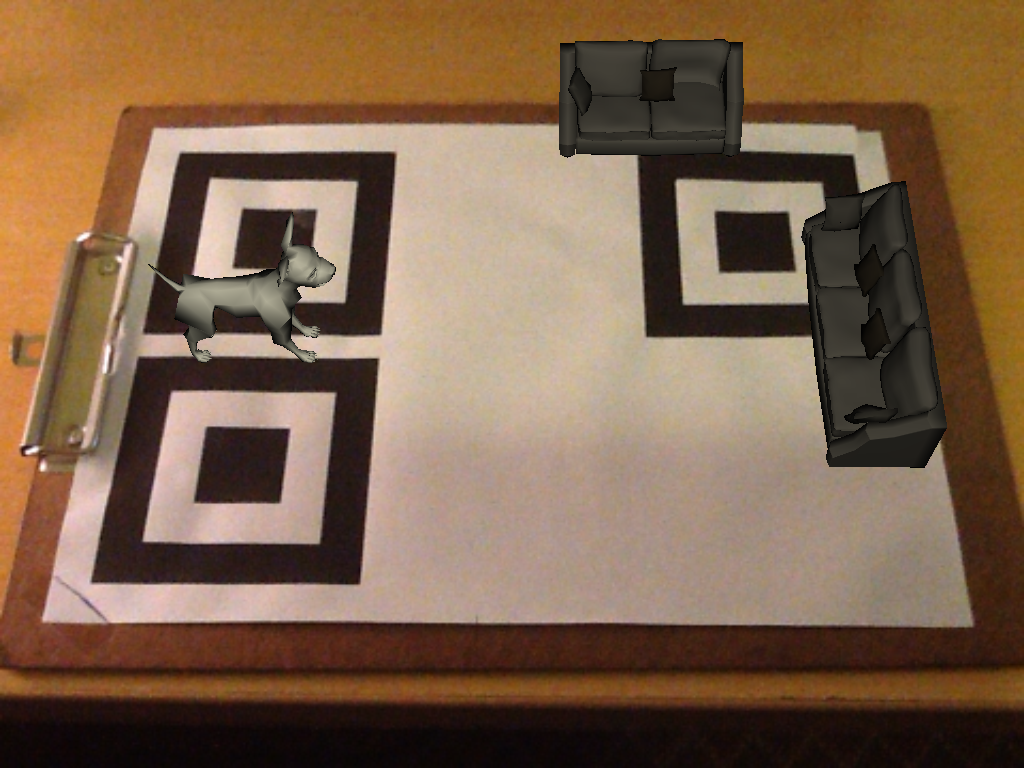
\includegraphics[scale=0.2]{figs_casosuso/CasoUso3_1.png} & 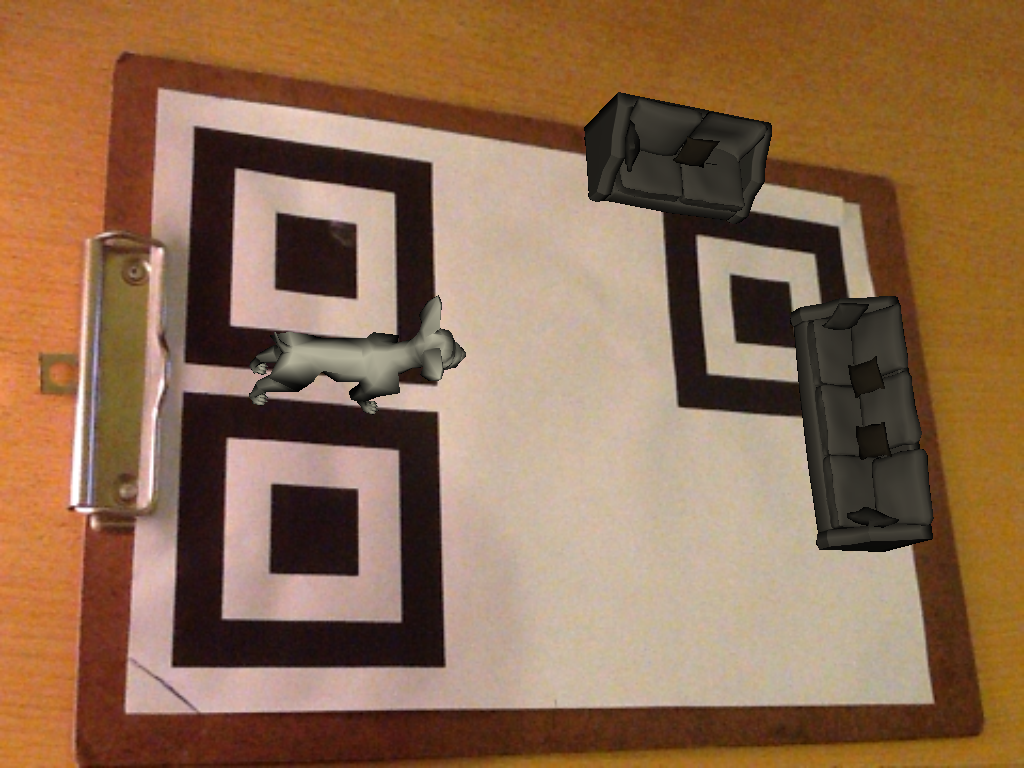
\includegraphics[scale=0.2]{figs_casosuso/CasoUso3_2.png}
\end{array}
$$
\caption{Dos capturas de pantalla del caso de uso ``modelos'', desde dos �ngulos disintos. Se pueden ver los modelos 3D pertenecientes a un perro chihuahue\~no y a dos sillones, uno de dos plazas y otro de tres.}
\label{fig:CasoUso3}
\end{figure}

\subsection{Detalles constructivos}
Los detalles constructivos de este caso de uso pueden consultarse en el Cap�tulo \ref{chap: render}.

\section{Resumen}

En este cap�tulo se present� la necesidad de contar con ciertos casos de uso que resolvieran cada uno de los desaf�os t�cnicos existentes en una aplicaci�n interactiva y de realidad aumentada completa para museos. Se definieron y describieron los tres casos de uso, y se mostraron algunas im�genes que ayudaran al lector a comprender el funcionamiento de cada uno de ellos. Adem�s, se definieron en cada caso, las herramientas t�cnicas extra necesarias para su implemenetaci�n.




\bibliographystyle{unsrt}   
\bibliography{encuadro}  
\end{document}
